\section{Introduction}
\label{sec:intro}
Opinions about a certain named entity,
such as a famous person, a world-wide organization, or a place,
may differ from culture to culture.
For example, \textit{Kashmir} is a large mountainous region on the China-India border.
Due to decades of border disputes between China and India
about that region, to the Chinese people, this region is
almost synonymous to military conflicts and political struggles.
On the contrary, that same region is considered as a picturesque travel
destination by the westerners due to its perfect location in the Himalayas,
since the border dispute between China and India is hardly their concern.
This type of cross-cultural differences of named entities are evident from the most popular
images about Kashmir on the English and Chinese search engines\footnote{Image search result from Bing on June 2017.}(see~\figref{fig:kashmir}).

%Another type of cross-cultural differences exist when an entity is interesting
%to one culture but largely ignored by another culture. \figref{fig:bjp}
%shows such an example where Indian People's Party
%(a.k.a. Bharatiya Janata Party or BJP), currently the largest political
%party in India, shows up frequently on Chinese web with vivid rally images,
%because India is a major world power that sits next to China and therefore Chinese media always concerns the events about BJP. 
%On the other hand, the most popular English web images about BJP are
%merely party logos, suggesting very little public interest about this
%entity from the English world.

%
%\begin{figure}[!ht]
%	\centering
%    \begin{subfigure}{0.30\columnwidth}
%        \centering
%        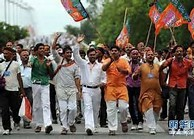
\includegraphics[width=\columnwidth]{yindu1.jpg}
%    \end{subfigure}
%    \begin{subfigure}{0.300\columnwidth}
%        \centering
%        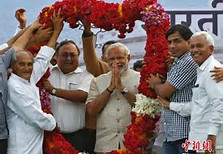
\includegraphics[width=\columnwidth]{yindu2.jpg}
%    \end{subfigure}
%	\begin{subfigure}{0.30\columnwidth}
%        \centering
%        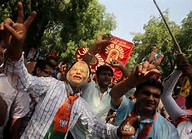
\includegraphics[width=\columnwidth]{yindu3.jpg}
%    \end{subfigure}
%	\centering
%    \begin{subfigure}{0.30\columnwidth}
%        \centering
%        
\includegraphics[width=\columnwidth]{bjp1.jpg}
%    \end{subfigure}
%    \begin{subfigure}{0.30\columnwidth}
%        \centering
%        
\includegraphics[width=\columnwidth]{bjp2.jpg}
%    \end{subfigure}
%	\begin{subfigure}{0.30\columnwidth}
%        \centering
%        
\includegraphics[width=\columnwidth]{bjp3.jpg}
%    \end{subfigure}
%	\caption{Popular Images about BJP on Chinese web (top) and
%English web (bottom)}
%	\label{fig:bjp}
%\end{figure}

Our goal in this paper is to identify an entity with significantly different
cultural understanding, which can contribute to applications such
as instant messenger or machine translator,
to avoid culturally sensitive mentions or translations.
Apart from these applications, a list of such entities with
cultural differences in its own right is a valuable resource for
cross-cultural studies.
However, understanding subtle cultural differences requires not
only perfect understanding of the two languages, but also devouring
large volumes of biligual texts to sufficiently observe how
they are mentioned in each culture and how they differ.
\begin{figure}[t]
	\vspace{10pt}
	\centering
	\begin{subfigure}{0.30\columnwidth}
		\centering
		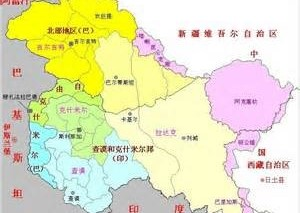
\includegraphics[width=\columnwidth]{keshimier1.jpg}
	\end{subfigure}
	\begin{subfigure}{0.30\columnwidth}
		\centering
		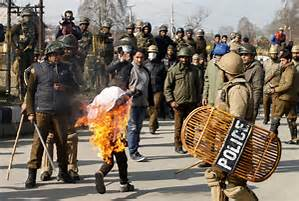
\includegraphics[width=\columnwidth]{keshimier2.jpg}
	\end{subfigure}
	\begin{subfigure}{0.30\columnwidth}
		\centering
		
\includegraphics[width=\columnwidth]{keshimier3.jpg}
	\end{subfigure}
	\centering
	\begin{subfigure}{0.30\columnwidth}
		\centering
		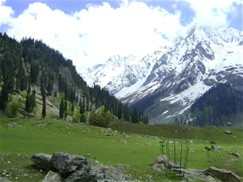
\includegraphics[width=\columnwidth]{kashmir1.jpg}
	\end{subfigure}
	\begin{subfigure}{0.30\columnwidth}
		\centering
		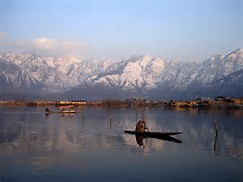
\includegraphics[width=\columnwidth]{kashmir2.jpg}
	\end{subfigure}
	\begin{subfigure}{0.30\columnwidth}
		\centering
		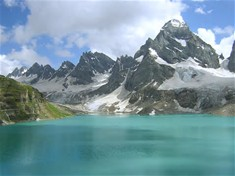
\includegraphics[width=\columnwidth]{kashmir3.jpg}
	\end{subfigure}
	\caption{Popular images about Kashmir on Chinese web (top) and
		English web (bottom) \vspace{5pt}}
	\label{fig:kashmir}
\end{figure}

We transform this problem into a computational task,
by proposing a quantitative evaluation metric measuring
the cultural similarity between two cultures of a given named entity.
To calculate such scores, we propose two approaches to compute
the cultural similarity scores based on the word embeddings trained in each mono-lingual corpus receptively.
The first solution connects the two results using linear transformation so that we can directly compute the cosine similarity between the English name and the Chinese name of a certain named entity.
Another way is to construct a higher-dimensional vector space.
Every dimension of this space is representing a pair of words,
which are an English word and its corresponding Chinese translation.
We call this space ``translation space''.
The values in the English name vector of a certain entity are
the cosine similarities between
this entity's English name and each of other English words.
We similarly compute the Chinese name vector.
Because an English word may has many different Chinese translations, we duplicate the cosine similarities into several dimensions in translation space. After constructing this new comprehensive vector space, we can simply calculate cosine similarity between the English and Chinese vector of a certain entity.

%The last method is also based on the comprehensive semantic space we just constructed, but we focus instead on the top K highest dimensions to calculate the Jaccard similarity between the two name of a certain entity.

%We proposed three algorithms calculating the scores, which are all based on word-embedding technique.
%Contribution
%
%This paper makes the following contributions:
%\begin{itemize}
%\item to the best of our knowledge, we are the first to study the problem
%of mining cultural differences of named entities and to present a data-driven
%approach to solve it;
%\item we applied our approach on large news corpora in English and Chinese and
%computed the cultural difference scores for 4,212 named entities including
%persons, locations and organizations from Wikipedia;
%\item our evaluation shows that the computed scores
%correlated well with human perception of cultural differences, with an
%average precision of 0.617 and 0.612,
%outperforming a strong baseline method using the popularities of entities by significant margins.
%%Spearman coefficient of 0.245 and Pearson coefficient of 0.229,
%\end{itemize}
